% Chapter Template

\chapter{Experiments} % Main chapter title

\label{Experiments} 


%----------------------------------------------------------------------------------------
%	SECTION 1
%----------------------------------------------------------------------------------------
\section{Experimental Setup}
This section covers the environment setup used for performing the experiments. Our experimental setup involved carrying out task-incremental learning with three tasks for each use case. The performance of the model in the task-incremental setting was evaluated using two settings:
\begin{enumerate}
\item \textbf{Baseline}: This involved performing sequential supervised fine-tuning and merging of LoRA adapters on three tasks. The details for this setting are provided in Section \ref{baseline_setup}.
\item \textbf{Mitigation}: This involved performing sequential supervised fine-tuning and merging of LoRA adapters with replay implementation. The details for this setting are provided in Section \ref{mitigation_setup}.
\end{enumerate}

To address our research questions \ref{RQ3} and \ref{RQ4}, we performed ablation studies with the order of tasks in the task-incremental learning setup. This ablation was performed for both Code Generation and Natural Language Generation use cases.
Additionally, for Code Generation use case, we performed an ablation study with a varying seed value.


\subsection{Experiment Environment}
All our experiments were carried out with the following hardware specifications and software environment. Python was used for development. The hardware and software configurations are shown in Table \ref{tab:hardware} and \ref{tab:software} respectively.

\begin{table}[h!]
\centering
\caption{Hardware Specifications.}
\label{tab:hardware}
\begin{tabular}{| m{4cm} | m{6cm} |}
\hline
\textbf{Component} & \textbf{Details} \\
\hline
GPU & NVIDIA H100 PCIE Tensor Core GPU \\
GPU memory & 80GB \\
\hline
\end{tabular}
\end{table}

\begin{table}[h!]
\centering
\caption{Software Environment.}
\label{tab:software}
\begin{tabular}{| m{4cm} | m{4cm} |}
\hline
\textbf{Component} & \textbf{Version} \\
\hline
Python & 3.11 \\
PyTorch & 2.2.1 \\
CUDA & 12.2 \\
Transformers & 4.41.0.dev0 \\
PEFT & 0.10.1.dev0 \\
TRL & 0.8.1 \\
Datasets & 2.18.0 \\
MLFlow & 2.11.3 \\
\hline
\end{tabular}
\end{table}
\subsection{Model Architectures}
We used DeepSeek-Coder-6.7B-Instruct model for the Code Generation use case and Llama-3-8B-Instruct model for the Natural Language Generation use case. Both of these models use the Llama architecture. The specifications for the models are shown in Table \ref{tab:specs}.

\begin{table}[h!]
\centering
\caption{Model Specifications.}
\label{tab:specs}
\begin{tabular}{| m{4cm} | m{5cm} | m{1.2cm} | m{1.2cm} | m{1.2cm} |}
\hline
\textbf{Model} & \textbf{Training Data} & \textbf{Params} & \textbf{Context Length} & \textbf{Token count} \\
\hline
DeepSeek-Coder-6.7B-Instruct & 87\% code and 13\% linguistic data in both English and Chinese languages. & 6.7B & 16K & 2T \\
\hline
Meta-Llama-3-8B-Instruct & A new mix of publicly available online data & 8B & 8K & 15T+ \\
\hline
\end{tabular}
\end{table}

\begin{figure}[h!]
    \centering
    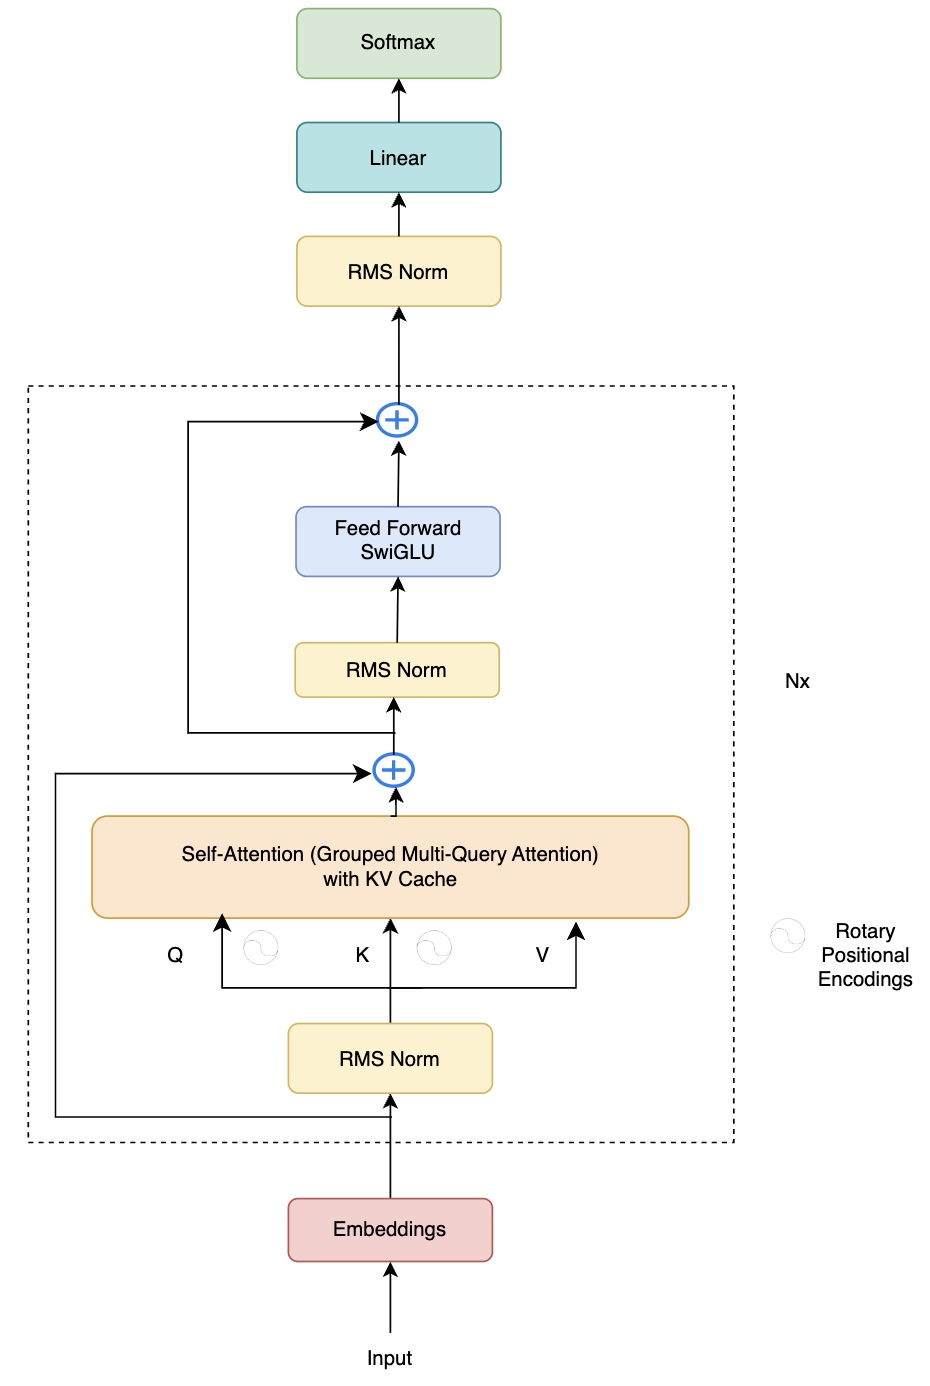
\includegraphics[width=0.88\textwidth]{Figures/experiments/llama_arch.jpeg} 
    \caption{Llama Architecture.}
    \label{fig:LlamaArch}
\end{figure}

Llama \cite{touvron2023llama} is an auto-regressive language model that uses an optimized transformer architecture. It uses Grouped Query Attention (GQA), RoPE (Rotary Positional Embeddings) used for Query and Key, RMS (Root Mean Squared Error) Normalization and KV Cache. 

\subsubsection{Grouped Multi-Query Attention} 
Grouped-query attention (GQA) is an interpolation of multi-query and multi-head attention. It performs similarly to multi-head attention while maintaining a speed similar to multi-query attention. Multi-Query Attention (MQA) is a process that uses only a single key-value head for multiple queries. This helps to save memory and fasten decoder inference. The Llama architecture uses GQA to overcome the memory bandwidth challenges faced during the autoregressive decoding of Transformer models.

\subsubsection{Rotary Positional Embeddings (RoPE)}
The Llama architecture uses a positional encoding mechanism called Rotary Positional Embeddings \cite{su2024roformer}. It works in the angular domain instead of using the weight of the direct position of the token. RoPE is used to transform or rotate the hidden state embedding at a certain angle. This angle is proportional to the position of the word in the sentence. RoPE is applied only to the query and keys but not the values. 

\subsubsection{Root Mean Squared Normalization (RMSNorm)}
Root Mean Square Normalization (RMSNorm) \cite{zhang2019root} is a normalization technique that ensures that the activations are consistently scaled regardless of the mini-batch size or the number of features. It focuses on re-scaling invariance and regularizes the summed inputs according to the Root Mean Square value. RMSNorm introduces learnable scale parameters, enabling adaptability similar to Batch Normalization.

\subsubsection{KV Cache}
KV Cache allows the model to perform less computation on tokens that it has already seen during inference. At each inference step, we only require the last token output by the model since we have the previous ones. However, the model needs access to all the previous tokens for context to decide which token to output. KV Cache helps the model remember the context in terms of intermediate outputs.

\subsection{Hyperparameters and Training Configuration}
For all our experiments, we trained the models with 3 epochs, a weight decay ratio of 0.001, and a cosine learning rate scheduler with a warmup ratio of 0.01. The data type was set to be bfloat16 and the maximum sequence length was set to 8192. 8 bit Paged AdamW optimizer was used and Flash Attention2 was used as the attention implementation. Different learning rates were used for each task. These learning rates were identified through experimentation. 

For the LoRA adapters, a rank value of 256 and an alpha value of 256 were used. The LoRA dropout to set to 0.01 and all linear layers were set to be the LoRA target modules: gate\_proj, down\_proj, up\_proj, q\_proj, v\_proj, k\_proj, and o\_proj using “all-linear”. 

Batch size per task were set to optimize for iterations per second as opposed to memory consumption so that runs would complete as fast as possible.

Learning rates were set by running tests to obtain rates that avoid over-fitting on the loss over 3 epochs given the batch size set for the test. The learning rates used for the different tasks are listed in Table \ref{tab:lr}.
\begin{table}[h!]
\centering
\caption{Learning rates used for different tasks.}
\label{tab:lr}
\begin{tabular}{| m{5cm} | m{6cm} | m{3cm} |}
\hline
\textbf{Use case} & \textbf{Task} & \textbf{Learning rate} \\
\hline
\multirow{3}{*}{Code Generation} & Code Generation in C++ & 2.5e-5 \\
& Unit Test Generation & 2.5e-5 \\
& Manifest Generation & 5e-5 \\
\hline
\multirow{3}{*}{Natural Language Generation} & Question Answering & 2.5e-7 \\
& Summarization & 5e-7 \\
& Mathematical Reasoning & 2.5e-7 \\
\hline
\end{tabular}
\end{table}

\section{Ablation studies}
To address research questions \ref{RQ3} and \ref{RQ4}, we conducted ablation studies to investigate the impact of task order in task-incremental instruction fine-tuning. The ablation studies involved varying the sequence of tasks for both Code Generation use case (\ref{RQ3a} and \ref{RQ4a}) and  Natural Language Generation use case (\ref{RQ3b} and \ref{RQ4b}). For each use case, we tested all possible permutations of task order for the three tasks, which resulted in six different fine-tuning sequences. We performed these task sequences for both the baseline and mitigation setups. This resulted in 12 fine-tuning sequences for each use case. These experiments allowed us to measure the retention of both the pre-trained model capabilities and the task-specific capabilities. Through this ablation study, we compared whether certain sequences lead to better model performances and retention of capabilities.

For code generation, an additional ablation study was performed with varying seed value. This study allowed us to investigate whether the results from the experiments are consistent even with other seed values. 

\subsection{Code Generation use case}
\subsubsection{Task order}
The fine-tuning sequences used for the ablation studies for the Code Generation use case are shown in Table \ref{tab:CodeTaskOrder}. These fine-tuning sequences were performed for both the baseline and mitigation setups.

\begin{table}[h!]
\centering
\caption{Ablation tasks distribution for Code Generation use case}
\label{tab:CodeTaskOrder}
\begin{tabular}{| m{2cm} | m{3.4cm} | m{3.4cm} | m{3.4cm} |}
\hline
\textbf{Ablation} & \textbf{Task 1} & \textbf{Task 2} & \textbf{Task 3} \\
\hline
Ablation 1 & Code Generation & Unit Test Generation & Manifest Generation \\
\hline
Ablation 2 & Code Generation & Manifest Generation & Unit Test Generation \\
\hline
Ablation 3 & Unit Test Generation & Code Generation & Manifest Generation \\
\hline
Ablation 4 & Unit Test Generation & Manifest Generation & Code Generation \\
\hline
Ablation 5 & Manifest Generation & Code Generation & Unit Test Generation \\
\hline
Ablation 6 & Manifest Generation & Unit Test Generation & Code Generation \\
\hline
\end{tabular}
\end{table}

\subsubsection{Seed value}
An additional ablation study with varying seed value was performed for code generation use case. Two seed values were used. The task order experiments with both the baseline and mitigation setups were performed for both seed values.

\subsection{Natural Language Generation use case}
The fine-tuning sequences used for the ablation studies for the Natural Language Generation use case are shown in Table \ref{tab:GenTaskOrder}. These fine-tuning sequences were performed for both the baseline and mitigation setups.
For the experiment runs for natural language use case, a single seed value was used.

\begin{table}[h!]
\centering
\caption{Ablation tasks distribution for Natural Language Generation use case}
\label{tab:GenTaskOrder}
\begin{tabular}{| m{1.8cm} | m{4.5cm} | m{4.5cm} | m{4.5cm} |}
\hline
\textbf{Ablation} & \textbf{Task 1} & \textbf{Task 2} & \textbf{Task 3} \\
\hline
Ablation 1 & Question Answering & Summarization & Mathematical Reasoning \\
\hline
Ablation 2 & Question Answering & Mathematical Reasoning & Summarization \\
\hline
Ablation 3 & Summarization & Question Answering & Mathematical Reasoning \\
\hline
Ablation 4 & Summarization & Mathematical Reasoning & Question Answering \\
\hline
Ablation 5 & Mathematical Reasoning & Question Answering & Summarization \\
\hline
Ablation 6 & Mathematical Reasoning & Summarization & Question Answering \\
\hline
\end{tabular}
\end{table}